
%% bare_jrnl.tex
%% V1.4b
%% 2015/08/26
%% by Michael Shell
%% see http://www.michaelshell.org/
%% for current contact information.B8-85-84-AF-15-1B
%%
%% This is a skeleton file demonstrating the use of IEEEtran.cls
%% (requires IEEEtran.cls version 1.8b or later) with an IEEE
%% journal paper.
%%
%% Support sites: %% http://www.michaelshell.org/tex/ieeetran/
%% http://www.ctan.org/pkg/ieeetran
%% and
%% http://www.ieee.org/

%%*************************************************************************
%% Legal Notice:
%% This code is offered as-is without any warranty either expressed or
%% implied; without even the implied warranty of MERCHANTABILITY or
%% FITNESS FOR A PARTICULAR PURPOSE!
%% User assumes all risk.
%% In no event shall the IEEE or any contributor to this code be liable for
%% any damages or losses, including, but not limited to, incidental,
%% consequential, or any other damages, resulting from the use or misuse
%% of any information contained here.
%%
%% All comments are the opinions of their respective authors and are not
%% necessarily endorsed by the IEEE.
%%
%% This work is distributed under the LaTeX Project Public License (LPPL)
%% ( http://www.latex-project.org/ ) version 1.3, and may be freely used,
%% distributed and modified. A copy of the LPPL, version 1.3, is included
%% in the base LaTeX documentation of all distributions of LaTeX released
%% 2003/12/01 or later.
%% Retain all contribution notices and credits.
%% ** Modified files should be clearly indicated as such, including  **
%% ** renaming them and changing author support contact information. **
%%*************************************************************************


% *** Authors should verify (and, if needed, correct) their LaTeX system  ***
% *** with the testflow diagnostic prior to trusting their LaTeX platform ***
% *** with production work. The IEEE's font choices and paper sizes can   ***
% *** trigger bugs that do not appear when using other class files.       ***                          ***
% The testflow support page is at:
% http://www.michaelshell.org/tex/testflow/



\documentclass[journal]{IEEEtran}
%
% If IEEEtran.cls has not been installed into the LaTeX system files,
% manually specify the path to it like:
% \documentclass[journal]{../sty/IEEEtran}





% Some very useful LaTeX packages include:
% (uncomment the ones you want to load)


% *** MISC UTILITY PACKAGES ***
%
%\usepackage{ifpdf}
% Heiko Oberdiek's ifpdf.sty is very useful if you need conditional
% compilation based on whether the output is pdf or dvi.
% usage:
% \ifpdf
%   % pdf code
% \else
%   % dvi code
% \fi
% The latest version of ifpdf.sty can be obtained from:
% http://www.ctan.org/pkg/ifpdf
% Also, note that IEEEtran.cls V1.7 and later provides a builtin
% \ifCLASSINFOpdf conditional that works the same way.
% When switching from latex to pdflatex and vice-versa, the compiler may
% have to be run twice to clear warning/error messages.






% *** CITATION PACKAGES ***
%
%\usepackage{cite}
% cite.sty was written by Donald Arseneau
% V1.6 and later of IEEEtran pre-defines the format of the cite.sty package
% \cite{} output to follow that of the IEEE. Loading the cite package will
% result in citation numbers being automatically sorted and properly
% "compressed/ranged". e.g., [1], [9], [2], [7], [5], [6] without using
% cite.sty will become [1], [2], [5]--[7], [9] using cite.sty. cite.sty's
% \cite will automatically add leading space, if needed. Use cite.sty's
% noadjust option (cite.sty V3.8 and later) if you want to turn this off
% such as if a citation ever needs to be enclosed in parenthesis.
% cite.sty is already installed on most LaTeX systems. Be sure and use
% version 5.0 (2009-03-20) and later if using hyperref.sty.
% The latest version can be obtained at:
% http://www.ctan.org/pkg/cite
% The documentation is contained in the cite.sty file itself.






% *** GRAPHICS RELATED PACKAGES ***
%
\ifCLASSINFOpdf
  % \usepackage[pdftex]{graphicx}
  % declare the path(s) where your graphic files are
  % \graphicspath{{../pdf/}{../jpeg/}}
  % and their extensions so you won't have to specify these with
  % every instance of \includegraphics
  % \DeclareGraphicsExtensions{.pdf,.jpeg,.png}
\else
  % or other class option (dvipsone, dvipdf, if not using dvips). graphicx
  % will default to the driver specified in the system graphics.cfg if no
  % driver is specified.
  % \usepackage[dvips]{graphicx}
  % declare the path(s) where your graphic files are
  % \graphicspath{{../eps/}}
  % and their extensions so you won't have to specify these with
  % every instance of \includegraphics
  % \DeclareGraphicsExtensions{.eps}
\fi
% graphicx was written by David Carlisle and Sebastian Rahtz. It is
% required if you want graphics, photos, etc. graphicx.sty is already
% installed on most LaTeX systems. The latest version and documentation
% can be obtained at:
% http://www.ctan.org/pkg/graphicx
% Another good source of documentation is "Using Imported Graphics in
% LaTeX2e" by Keith Reckdahl which can be found at:
% http://www.ctan.org/pkg/epslatex
%
% latex, and pdflatex in dvi mode, support graphics in encapsulated
% postscript (.eps) format. pdflatex in pdf mode supports graphics
% in .pdf, .jpeg, .png and .mps (metapost) formats. Users should ensure
% that all non-photo figures use a vector format (.eps, .pdf, .mps) and
% not a bitmapped formats (.jpeg, .png). The IEEE frowns on bitmapped formats
% which can result in "jaggedy"/blurry rendering of lines and letters as
% well as large increases in file sizes.
%
% You can find documentation about the pdfTeX application at:
% http://www.tug.org/applications/pdftex


\usepackage{color}
\usepackage{amsmath}
\usepackage{amssymb}
\usepackage{tabularx}

\usepackage{epsfig}
%\usepackage[colorlinks=false, urlcolor=black, pdfborder={0 0 0}]{hyperref}
%\let\url\nolinkurl
%\usepackage[options]{nohyperref}  % This makes hyperref commands do nothing without errors
\usepackage{url}  % This makes \url work

%\usepackage[dvips]{epsfig}
\usepackage{etoolbox}
\apptocmd{\sloppy}{\hbadness 10000\relax}{}{}

\usepackage{longtable}
\usepackage{graphicx}
\usepackage[T1]{fontenc}
\usepackage{paralist}
\usepackage{enumitem}
%%%%%%%%%%%%for
\usepackage{adjustbox}
\usepackage{array}
\usepackage{booktabs}
\newcolumntype{C}{>{\centering\arraybackslash}X} % centered version of "X" type
\setlength{\extrarowheight}{1pt}
%\usepackage{lipsum}
\usepackage{multirow}

\newcolumntype{R}[2]{%
    >{\adjustbox{angle=#1,lap=\width-(#2)}\bgroup}%
    l%
    <{\egroup}%
}
\newcommand*\rot{\multicolumn{1}{R{45}{1em}}}% no optional argument here, please!

\usepackage{epstopdf}


\def\BibTeX{{\rm B\kern-.05em{\sc i\kern-.025em b}\kern-.08em
    T\kern-.1667em\lower.7ex\hbox{E}\kern-.125emX}}

\usepackage{pdflscape}
%\usepackage{subfigure}
\usepackage{tabularx}
\usepackage{xtab}
%\usepackage{supertabular}

\usepackage{booktabs, threeparttable}
\usepackage{array}
\newcolumntype{L}[1]{>{\raggedright\arraybackslash}p{#1}}

% *** MATH PACKAGES ***
\usepackage{algorithm}
\usepackage[noend]{algpseudocode}

\makeatletter
\def\BState{\State\hskip-\ALG@thistlm}
\makeatother

\algnewcommand\algorithmicswitch{\textbf{switch}}
\algnewcommand\algorithmiccase{\textbf{case}}
\algnewcommand\algorithmicassert{\texttt{assert}}
\algnewcommand\Assert[1]{\State \algorithmicassert(#1)}%
% New "environments"
\algdef{SE}[SWITCH]{Switch}{EndSwitch}[1]{\algorithmicswitch\ #1\ \algorithmicdo}{\algorithmicend\ \algorithmicswitch}%
\algdef{SE}[CASE]{Case}{EndCase}[1]{\algorithmiccase\ #1}{\algorithmicend\ \algorithmiccase}%
\algtext*{EndSwitch}%
\algtext*{EndCase}%





% *** SPECIALIZED LIST PACKAGES ***
%
%\usepackage{algorithmic}
% algorithmic.sty was written by Peter Williams and Rogerio Brito.
% This package provides an algorithmic environment fo describing algorithms.
% You can use the algorithmic environment in-text or within a figure
% environment to provide for a floating algorithm. Do NOT use the algorithm
% floating environment provided by algorithm.sty (by the same authors) or
% algorithm2e.sty (by Christophe Fiorio) as the IEEE does not use dedicated
% algorithm float types and packages that provide these will not provide
% correct IEEE style captions. The latest version and documentation of
% algorithmic.sty can be obtained at:
% http://www.ctan.org/pkg/algorithms
% Also of interest may be the (relatively newer and more customizable)
% algorithmicx.sty package by Szasz Janos:
% http://www.ctan.org/pkg/algorithmicx




% *** ALIGNMENT PACKAGES ***
%
%\usepackage{array}
% Frank Mittelbach's and David Carlisle's array.sty patches and improves
% the standard LaTeX2e array and tabular environments to provide better
% appearance and additional user controls. As the default LaTeX2e table
% generation code is lacking to the point of almost being broken with
% respect to the quality of the end results, all users are strongly
% advised to use an enhanced (at the very least that provided by array.sty)
% set of table tools. array.sty is already installed on most systems. The
% latest version and documentation can be obtained at:
% http://www.ctan.org/pkg/array


% IEEEtran contains the IEEEeqnarray family of commands that can be used to
% generate multiline equations as well as matrices, tables, etc., of high
% quality.




% *** SUBFIGURE PACKAGES ***
%\ifCLASSOPTIONcompsoc
%  \usepackage[caption=false,font=normalsize,labelfont=sf,textfont=sf]{subfig}
%\else
%  \usepackage[caption=false,font=footnotesize]{subfig}
%\fi
% subfig.sty, written by Steven Douglas Cochran, is the modern replacement
% for subfigure.sty, the latter of which is no longer maintained and is
% incompatible with some LaTeX packages including fixltx2e. However,
% subfig.sty requires and automatically loads Axel Sommerfeldt's caption.sty
% which will override IEEEtran.cls' handling of captions and this will result
% in non-IEEE style figure/table captions. To prevent this problem, be sure
% and invoke subfig.sty's "caption=false" package option (available since
% subfig.sty version 1.3, 2005/06/28) as this is will preserve IEEEtran.cls
% handling of captions.
% Note that the Computer Society format requires a larger sans serif font
% than the serif footnote size font used in traditional IEEE formatting
% and thus the need to invoke different subfig.sty package options depending
% on whether compsoc mode has been enabled.
%
% The latest version and documentation of subfig.sty can be obtained at:
% http://www.ctan.org/pkg/subfig




% *** FLOAT PACKAGES ***
%
%\usepackage{fixltx2e}
% fixltx2e, the successor to the earlier fix2col.sty, was written by
% Frank Mittelbach and David Carlisle. This package corrects a few problems
% in the LaTeX2e kernel, the most notable of which is that in current
% LaTeX2e releases, the ordering of single and double column floats is not
% guaranteed to be preserved. Thus, an unpatched LaTeX2e can allow a
% single column figure to be placed prior to an earlier double column
% figure.
% Be aware that LaTeX2e kernels dated 2015 and later have fixltx2e.sty's
% corrections already built into the system in which case a warning will
% be issued if an attempt is made to load fixltx2e.sty as it is no longer
% needed.
% The latest version and documentation can be found at:
% http://www.ctan.org/pkg/fixltx2e


%\usepackage{stfloats}
% stfloats.sty was written by Sigitas Tolusis. This package gives LaTeX2e
% the ability to do double column floats at the bottom of the page as well
% as the top. (e.g., "\begin{figure*}[!b]" is not normally possible in
% LaTeX2e). It also provides a command:
%\fnbelowfloat
% to enable the placement of footnotes below bottom floats (the standard
% LaTeX2e kernel puts them above bottom floats). This is an invasive package
% which rewrites many portions of the LaTeX2e float routines. It may not work
% with other packages that modify the LaTeX2e float routines. The latest
% version and documentation can be obtained at:
% http://www.ctan.org/pkg/stfloats
% Do not use the stfloats baselinefloat ability as the IEEE does not allow
% \baselineskip to stretch. Authors submitting work to the IEEE should note
% that the IEEE rarely uses double column equations and that authors should try
% to avoid such use. Do not be tempted to use the cuted.sty or midfloat.sty
% packages (also by Sigitas Tolusis) as the IEEE does not format its papers in
% such ways.
% Do not attempt to use stfloats with fixltx2e as they are incompatible.
% Instead, use Morten Hogholm'a dblfloatfix which combines the features
% of both fixltx2e and stfloats:
%
% \usepackage{dblfloatfix}
% The latest version can be found at:
% http://www.ctan.org/pkg/dblfloatfix




%\ifCLASSOPTIONcaptionsoff
%  \usepackage[nomarkers]{endfloat}
% \let\MYoriglatexcaption\caption
% \renewcommand{\caption}[2][\relax]{\MYoriglatexcaption[#2]{#2}}
%\fi
% endfloat.sty was written by James Darrell McCauley, Jeff Goldberg and
% Axel Sommerfeldt. This package may be useful when used in conjunction with
% IEEEtran.cls'  captionsoff option. Some IEEE journals/societies require that
% submissions have lists of figures/tables at the end of the paper and that
% figures/tables without any captions are placed on a page by themselves at
% the end of the document. If needed, the draftcls IEEEtran class option or
% \CLASSINPUTbaselinestretch interface can be used to increase the line
% spacing as well. Be sure and use the nomarkers option of endfloat to
% prevent endfloat from "marking" where the figures would have been placed
% in the text. The two hack lines of code above are a slight modification of
% that suggested by in the endfloat docs (section 8.4.1) to ensure that
% the full captions always appear in the list of figures/tables - even if
% the user used the short optional argument of \caption[]{}.
% IEEE papers do not typically make use of \caption[]'s optional argument,
% so this should not be an issue. A similar trick can be used to disable
% captions of packages such as subfig.sty that lack options to turn off
% the subcaptions:
% For subfig.sty:
% \let\MYorigsubfloat\subfloat
% \renewcommand{\subfloat}[2][\relax]{\MYorigsubfloat[]{#2}}
% However, the above trick will not work if both optional arguments of
% the \subfloat command are used. Furthermore, there needs to be a
% description of each subfigure *somewhere* and endfloat does not add
% subfigure captions to its list of figures. Thus, the best approach is to
% avoid the use of subfigure captions (many IEEE journals avoid them anyway)
% and instead reference/explain all the subfigures within the main caption.
% The latest version of endfloat.sty and its documentation can obtained at:
% http://www.ctan.org/pkg/endfloat
%
% The IEEEtran \ifCLASSOPTIONcaptionsoff conditional can also be used
% later in the document, say, to conditionally put the References on a
% page by themselves.




% *** PDF, URL AND HYPERLINK PACKAGES ***
%
%\usepackage{url}
% url.sty was written by Donald Arseneau. It provides better support for
% handling and breaking URLs. url.sty is already installed on most LaTeX
% systems. The latest version and documentation can be obtained at:
% http://www.ctan.org/pkg/url
% Basically, \url{my_url_here}.




% *** Do not adjust lengths that control margins, column widths, etc. ***
% *** Do not use packages that alter fonts (such as pslatex).         ***
% There should be no need to do such things with IEEEtran.cls V1.6 and later.
% (Unless specifically asked to do so by the journal or conference you plan
% to submit to, of course. )


% correct bad hyphenation here
%\hyphenation{op-tical net-works semi-conduc-tor}


\begin{document}
%
% paper title
% Titles are generally capitalized except for words such as a, an, and, as,
% at, but, by, for, in, nor, of, on, or, the, to and up, which are usually
% not capitalized unless they are the first or last word of the title.
% Linebreaks \\ can be used within to get better formatting as desired.
% Do not put math or special symbols in the title.
\title{Decentralised Reinforcement Learning in Fog-based Internet-of-Things}
%
%
% author names and IEEE memberships
% note positions of commas and nonbreaking spaces ( ~ ) LaTeX will not break
% a structure at a ~ so this keeps an author's name from being broken across
% two lines.
% use \thanks{} to gain access to the first footnote area
% a separate \thanks must be used for each paragraph as LaTeX2e's \thanks
% was not built to handle multiple paragraphs
%

\author{XXX~YYYY,
        and~ XXX~ZZZZ% <-this % stops a space
%\thanks{B. Omoniwa is with National Mathematical Centre, PMB 118, Abuja-Nigeria, email: tunjiomoniwa@gmail.com.}% <-this % stops a space

\thanks{Manuscript received March 14, 2019; revised July X, 2019.}
\thanks{Copyright (c) 2012 IEEE. Personal use of this material is permitted. However, permission to use this material for any other purposes must be obtained from the IEEE by sending a request to pubs-permissions@ieee.org.}
}

% note the % following the last \IEEEmembership and also \thanks -
% these prevent an unwanted space from occurring between the last author name
% and the end of the author line. i.e., if you had this:
%
% \author{....lastname \thanks{...} \thanks{...} }
%                     ^------------^------------^----Do not want these spaces!
%
% a space would be appended to the last name and could cause every name on that
% line to be shifted left slightly. This is one of those "LaTeX things". For
% instance, "\textbf{A} \textbf{B}" will typeset as "A B" not "AB". To get
% "AB" then you have to do: "\textbf{A}\textbf{B}"
% \thanks is no different in this regard, so shield the last } of each \thanks
% that ends a line with a % and do not let a space in before the next \thanks.
% Spaces after \IEEEmembership other than the last one are OK (and needed) as
% you are supposed to have spaces between the names. For what it is worth,
% this is a minor point as most people would not even notice if the said evil
% space somehow managed to creep in.



% The paper headers
\markboth{IEEE Internet of Things Journal,~Vol.~X, No.~X, August~2019}%
{YYYY \MakeLowercase{\textit{et al.}}: Decentralised Reinforcement Learning in Fog-based Internet-of-Things}
% The only time the second header will appear is for the odd numbered pages
% after the title page when using the twoside option.
%
% *** Note that you probably will NOT want to include the author's ***
% *** name in the headers of peer review papers.                   ***
% You can use \ifCLASSOPTIONpeerreview for conditional compilation here if
% you desire.




% If you want to put a publisher's ID mark on the page you can do it like
% this:
%\IEEEpubid{0000--0000/00\$00.00~\copyright~2015 IEEE}
% Remember, if you use this you must call \IEEEpubidadjcol in the second
% column for its text to clear the IEEEpubid mark.



% use for special paper notices
%\IEEEspecialpapernotice{(Invited Paper)}



% make the title area
\maketitle

% As a general rule, do not put math, special symbols or citations
% in the abstract or keywords.
\begin{abstract}
Reinforcement learning (RL) algorithms offers more insights about the overall futuristic functionalities for intelligent Internet-of-Things (IoT) devices. With the explosive growth in the number of IoT devices, as well as the highly-distributed deployments of these devices today, managing the IoT devices centrally becomes infeasible. As such, several disruptive paradigms have emerged, one of which is the fog computing-based IoT, which aim towards shifting computation, control, and decision-making closer to the network edge. However, mobility and power-constrain of these fog devices remains an issue of concern. In this paper, we apply a decentralized q-learning algorithm to minimize the communication outage cost and optimize energy utilization within a fog-based IoT network. Our proposed approach out-performs the results from previous works by guaranteeing reliable delivery of data and minimizing overall energy cost within the network. Our future work will take into consideration fairness and latency within the fog-based IoT system.
\end{abstract}

% Note that keywords are not normally used for peerreview papers.
\begin{IEEEkeywords}
Reinforcement learning (RL), Fog-based Internet-of-Things (IoT), q-learning, communication outage, energy management.
\end{IEEEkeywords}


% For peer review papers, you can put extra information on the cover
% page as needed:
% \ifCLASSOPTIONpeerreview
% \begin{center} \bfseries EDICS Category: 3-BBND \end{center}
% \fi
%
% For peerreview papers, this IEEEtran command inserts a page break and
% creates the second title. It will be ignored for other modes.
\IEEEpeerreviewmaketitle

\section{Background}
\IEEEPARstart{T}{he} fog/edge computing-based IoT (FECIoT) paradigm aims at moving computation, control, and decision-making within the IoT ecosystem closer to the network edge~\cite{Omoniwa2018}. Due to the limited range and power of IoT end-devices, mobile fog devices (which are often energy-constrained) will drive the FECIoT paradigm by forwarding sensed IoT data from source to destination. From reducing operational cost to improving channel reliability and load balancing, the mobile fog relays will play an important role in improving the overall network performance~\cite{BenMimoune2017}. The deployment and efficient utilization of these mobile fog devices as relays will contribute to the success of future IoT systems~\cite{Chiangh2016}, one of which is to overcome communication outages due to obstacles or long distances between a source (IoT sensor) and a remote destination node (where localized IoT services may be rendered).

However, in order for devices to communicate efficiently with minimal outage (loss of transmitted packets), several bottlenecks needs to be addressed, one of which is the inefficient utilization of energy by power-constrained mobile fog devices. For instance, energy can be used up when these devices actively communicate with neighbouring devices within the network, conversely, energy can be saved when the devices regulate their transmission by entering a passive mode, especially in situations when there are redundant relays that can convey same information. Furthermore, if multiple fog relays are in an active mode and unintelligently keep forwarding same message from an IoT end-device to a remote destination, soon they may run out of energy and die-out, hence, resulting in communication breakdown due to a point-of-failure within the network.

\begin{figure}[!t]
\centering
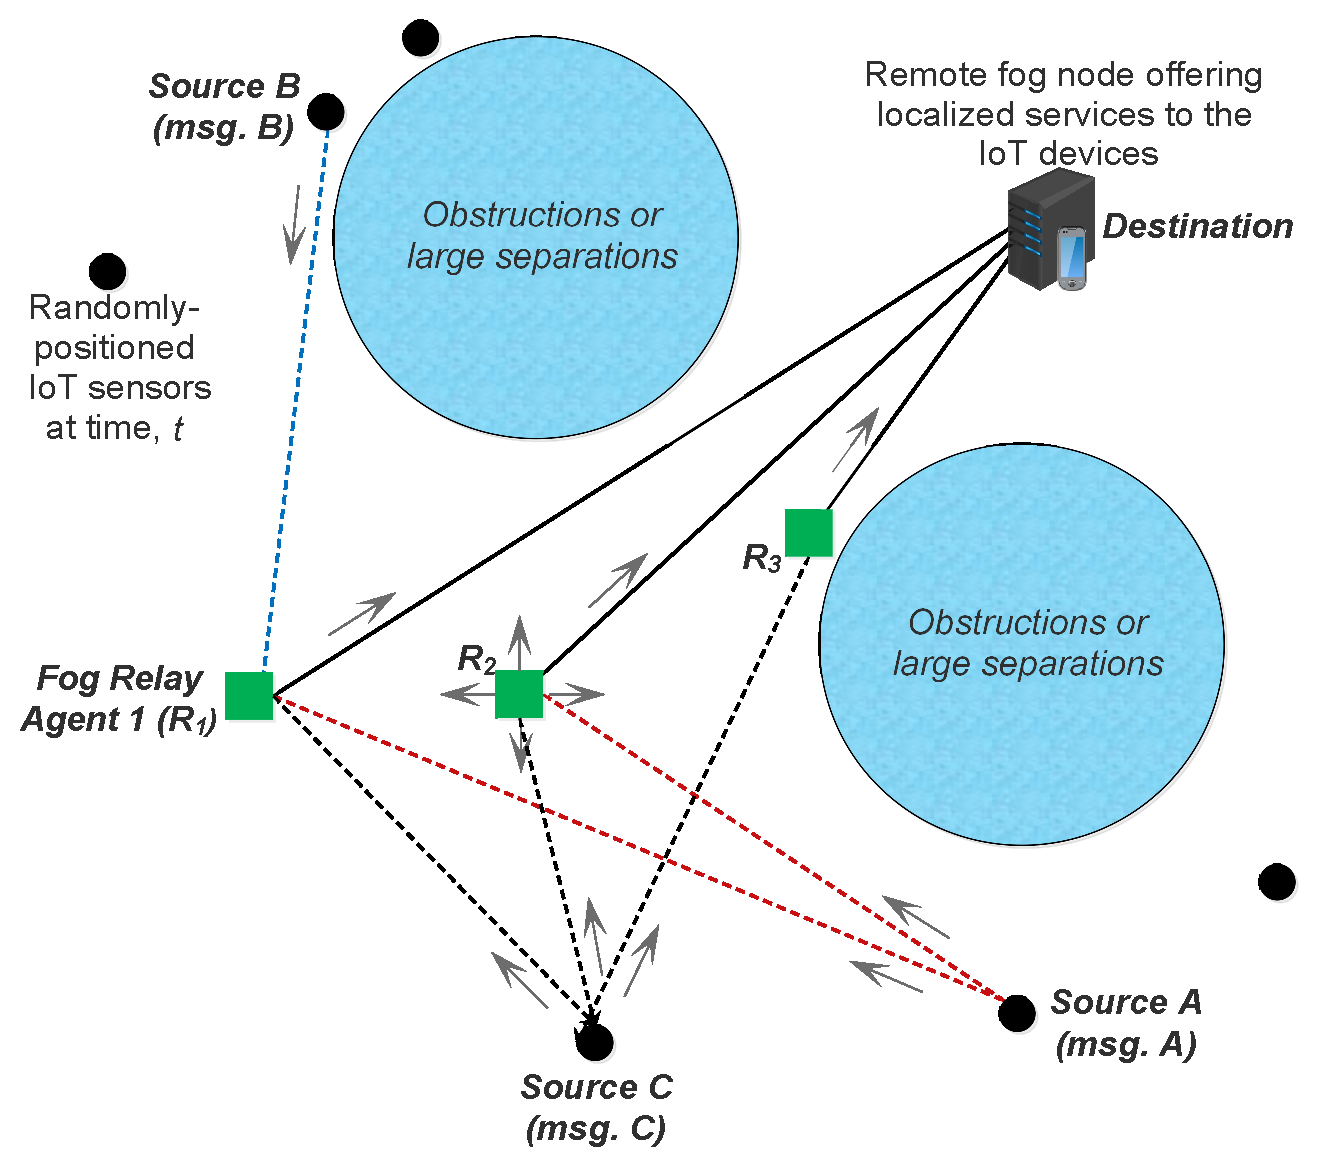
\includegraphics[width=3.2in]{ideafig1.eps}
 %where an .eps filename suffix will be assumed under latex,
% and a .pdf suffix will be assumed for pdflatex; or what has been declared
% via \DeclareGraphicsExtensions.
\caption{System model.}
\label{ideafig1}
\end{figure}

\begin{table*}
 \small
\centering
\caption{Classifications of Some Problems Addressed in Related Works}
\label{table:classification}
  \begin{tabular}{l|lllllllllll}
  \hline
 \textit{Reference} & \rot{\textit{Energy}} & \rot{\textit{Outage}} & \rot{\textit{Selection}} & \rot{\textit{Mobility}} & \rot{\textit{Latency}} & \rot{\textit{Traffic}} & \rot{\textit{Sources}} & \rot{\textit{Relays}} & \rot{\textit{Destination}} & \textit{Objective} & \textit{Approach} \\
  \hline \hline
   Omoniwa \emph{et al.}~\cite{OmoniwaRelay2018} & - & \checkmark & \checkmark & \checkmark & - & - & 1 & M & 1 & QoS & \multicolumn{1}{m{4cm}}{Steepest Descent method} \\ \hline
   Simiscuka \emph{et al.}~\cite{Simiscuka2018} & - & \checkmark & \checkmark  & - & \checkmark & - & M & M & M & QoS & \multicolumn{1}{m{4cm}}{Re-clustering Algorithm}\\ \hline
   Alsharoa \emph{et al.}~\cite{Alsharoa2018} & \checkmark & - & - & - & - & - & M & M & 1 & \multicolumn{1}{m{4cm}}{Energy, Relay planning} & \multicolumn{1}{m{4cm}}{Genetic Algorithm}\\ \hline
   Manzoor \emph{et al.}~\cite{Manzoor2018} & - & - & \checkmark & \checkmark & - & - & M & 1 & 1 & \multicolumn{1}{m{4cm}}{Relay selection} & Prototype design \\ \hline
    Lv \emph{et al.}~\cite{Lv2018} & \checkmark  & - & - & - & - & - & 1 & M & M & \multicolumn{1}{m{4cm}}{Energy} & Numerical \\ \hline
    Kawabata \emph{et al.}~\cite{Kawabata2017}  & - & \checkmark & \checkmark & - & - & - & M & M & M & QoS & \multicolumn{1}{m{4cm}}{Stochastic geometry}\\ \hline
    Behdad \emph{et al.}~\cite{Behdad2018} &  \checkmark & - & - & - & \checkmark & \checkmark & 1 & 1 & 1 & Energy, Latency, Conjestion & Analytical \\ \hline
     Our approach & \checkmark & \checkmark & \checkmark & \checkmark & - & - & M & M & M & QoS, Energy & \multicolumn{1}{m{4cm}}{Decentralized Q-learning} \\
      \hline \hline
 \end{tabular}
 \end{table*}

The FECIoT paradigm leverages on mobile fog devices, such as robots, drones, smart phones, smart watches, etc., to offer localized services to IoT end-devices. However, these devices are at risk of draining most of their energy when they move. As such, power-control mechanisms and smart mobility are critical in minimizing outages in communication, as well as optimizing energy utilization. This is crucial to drive several smart cities applications, most importantly the Industrial IoT (IIoT), where industrial robots are deployed in a dynamic industrial setting, and intelligent monitoring applications, where surveillance drones are deployed in militarised zones to meet stringent quality-of-service (QoS) requirements~\cite{OmoniwaRelay2018}.

Several relay-based works have tried to address the issue of communication outages~\cite{OmoniwaRelay2018},~\cite{Simiscuka2018},~\cite{Kawabata2017}, energy usage~\cite{Alsharoa2018},~\cite{Lv2018},~\cite{Behdad2018}, relay selection~\cite{OmoniwaRelay2018},~\cite{Simiscuka2018},~\cite{Manzoor2018},~\cite{Kawabata2017}, mobility~\cite{OmoniwaRelay2018},~\cite{Manzoor2018}, latency~\cite{Simiscuka2018},~\cite{Behdad2018} and congestion~\cite{Behdad2018} within the IoT ecosystem. However, these works considered centralized approaches which are prone to several challenges. Such challenges include scalability, failure or downtime in the central entity, overhead resulting from periodic updates and synchronization of nodes with the central controller often leading to inefficient energy utilization and decreased communication performance within the network.

The closest RL-based works were~\cite{Wilhelmi2017} and~\cite{Azari2018}, however these works focused on improving communication performance using the multi-armed bandit approach, which does not consider state transitions. On the other hand, our work model a realistic scenario of the defined problem and most importantly, applied a decentralized Q-learning approach with well-defined states, actions, and rewards.

%Considering the highly-distributed nature of deployed IoT devices, it becomes infeasible to manage devices centrally~\cite{Wilhelmi2017}. As such, reinforcement learning can be effectively deployed on fog devices to allow them to act independently based on their local experiences in the environment, i.e. each fog device should be able to learn independently without a central entity.
%
%A decentralised stateless Q-learning approach was proposed in \cite{Wilhelmi2017} to improve aggregate throughput in four coexistent wireless networks (WN). Each WN was considered to be an agent running the stateless Q-learning algorithm with agents having action space as channel number, and transmit power
%(dBm). A lightweight distributed learning approach was proposed in \cite{Azari2018} to increase energy efficiency and reliability of IoT communications. There was significant performance improvement when the proposed algorithm was compared to a centralized optimized strategy. Transmit power, sub-channel, and spreading factor made up the action space. However, the system model in both works was rather hierarchical than distributed, ie. each WN was assumed to be an independent central entity with no specifications to what is learnt within each sub-network. Though IoT is defined as a large-scale network where various sub-networks coexist~\cite{Omoniwa2018}, applying RL to end-devices within sub-network may bring about meaningful performance improvement in the overall IoT network.

The main contribution of our paper are summarized below:
\begin{enumerate}
  \item To apply a decentralised reinforcement learning approach as in~\cite{Gueriau2018} to optimize the communication performance within a fog-based IoT architecture.
  \item To optimize energy utilization within the network, taking into consideration the death of agents within the IoT network, hence making our decentralized approach robust to failure as compared to the centralized approaches.
  \item Taking into account mobility of the fog relays, we propose an efficient RL-based selection strategy where an active fog relay is selected for a particular transmission phase from a set of available potential fog relays.
\end{enumerate}

The remainder of this work is organized as follows.~In Section II, we reviewed related works, and present our proposed approach in Section III. In Section IV, we evaluate the proposed fog-based IoT system, and present the results in Section V. Section VI concludes the paper and outlines future directions.

\section{Related Works}
In Table \ref{table:classification}, we highlight some related works that address some of the key challenges within a relay-based IoT network.
Several works have tried to address the issue of communication outages~\cite{OmoniwaRelay2018},~\cite{Simiscuka2018},~\cite{Kawabata2017}, energy usage~\cite{Alsharoa2018},~\cite{Lv2018},~\cite{Behdad2018}, relay selection~\cite{OmoniwaRelay2018},~\cite{Simiscuka2018},~\cite{Manzoor2018},~\cite{Kawabata2017}, mobility~\cite{OmoniwaRelay2018},~\cite{Manzoor2018}, latency~\cite{Simiscuka2018},~\cite{Behdad2018} and congestion~\cite{Behdad2018} within the IoT ecosystem.
\begin{enumerate}[label=\alph*)]
  \item \emph{Outage in communication}: An iterative algorithm based on the steepest descent method was proposed in~\cite{OmoniwaRelay2018} to optimize communication performance in a multi-tier fog-based IoT architecture, where a fog device acts as an amplify and forward relay of received information from an IoT sensor to a higher hierarchically-placed destination fog device, which offers some localized services. In \cite{Simiscuka2018}, a relay and mobility scheme for IoT (REMOS-IoT) was proposed to improve the network QoS by effective resource management and decision-making. The centralized REMOS-IoT algorithm introduced also considered the mobility of fog gateways/relays in improving the network throughput without considering the efficient utilization of energy of these power-constrained IoT end-devices.
  \item \emph{Energy utilization}: An energy-efficient relaying scheme for IoT communications was presented in \cite{Alsharoa2018} to minimize energy consumption within an IoT network by solving the relay planning and QoS problems. A genetic algorithm-based approach was used to arrive at a sub-optimal low-complexity solution. Using numerical methods, the authors in \cite{Lv2018} considered the energy-efficient design of a multi-pair decode-and-forward relay-based IoT network, in which multiple sources simultaneously transmit their information to the corresponding destinations via a relay equipped with a large array.
  \item \emph{Relay selection}: The authors in \cite{Manzoor2018} designed a prototype, a mobile relay architecture for low-power IoT devices, which exploits third-party unknown mobile relays for the forwarding of medical data generated by BLE sensors to some central server in the cloud. In \cite{Kawabata2017}, a relay selection scheme for large-scale energy-harvesting IoT networks was proposed. The work applied a stochastic geometric approach and attempts to minimize the outage probability using a novel energy harvesting (EH) relay selection scheme.
\end{enumerate}

However, most of these works considered centralized approaches, which may not be suitable within the IoT domain due to several challenges. These challenges are listed below.
\begin{enumerate}
  \item A possible operational failure in the central controller may have drastic consequences on the entire network.
  \item It takes time for the central entity to become aware of unavailable relay nodes due to mobility, death or departure of these nodes.
  \item Managing energy usage of devices centrally is a complex task.
  \item Signaling overhead between the central controller and network devices may result in increased energy cost within the IoT network.
\end{enumerate}

The work in \cite{Wilhelmi2017} proposed a decentralized stateless variation of Q-learning to improve aggregate throughput in four coexistent wireless networks (WN). The approach used in the work was a variant of a multi-armed bandit approach as only actions an rewards were defined, however, the Q-learning update function used in the work was modified, and excluded state transitions. Similarly, a MAB approach was presented in \cite{Azari2018}, (which is a single-state RL-based algorithm with no state transitions) where the agent only observes rewards based on actions taken. Both works may not be suitable to model a realistic IoT environment as defined in our paper, which takes into consideration mobility, death, energy utilization and communication performance in the system.

We present a decentralised reinforcement learning approach that adequately addresses some key performance issues within the IoT domain. The focus of our work is to minimize outage in communication in a fog-based IoT network as shown in Fig. \ref{ideafig1}, minimize energy cost by active fog relays, and present an efficient RL-based selection strategy where an active fog relay is selected for a particular transmission phase from a set of available potential mobile fog relays. Unlike the centralized approaches considered in \cite{OmoniwaRelay2018} -- \cite{Behdad2018}, we present a decentralized autonomous system that is robust to failure, allowing agents to take independent actions and decisions.
Furthermore, we applied the Q-learning algorithm on the defined problem. To the best of our knowledge, this is the first work that applies Q-learning to a fog-based IoT network.


\section{Problem Definition}
In this section, we provide a full description of the system model, as well the RL approach used to address the problem. In Fig. \ref{ideafig1}, we show a network topology at time~$t$ where some randomly deployed IoT sensors have data/service request to send to remote destinations via some mobile fog relay agents (MFRA). We depict a realistic scenario where sensors may at some point in time be unable to reach the destination via all available MFRA due to long separation or obstructions between source and destination. We observe that source A can reach the local server via two MFRA, source B via a MFRA, and source C via three MFRA. As such, we try as much as possible to capture the features of the MFRA and its environment.

\subsection{MFRA environment}
\emph{States}: The states are defined as a tuple, $\langle$Outage communication cost ($\mathcal{P}_{out}$) /Energy status of the fog relay (J) /Neighbour potential to relay message (Availability of redundant nodes)$\rangle$.

\begin{itemize}
  \item \emph{Outage communication cost}: Outage observations from the environment is estimated using (\ref{eqn1a}) from \cite{OmoniwaRelay2018}, which gives an estimate of the communication outage when the agent takes an action, such as changing power levels or location, or both.
  \item \emph{Energy expended by fog relay}: This observation gives the agent insight on how much energy by the fog agent when following policy~$\omega_i \in \omega_{fog}$. If the fog agent continues to take sub-optimal actions, it depletes its energy and dies out.
  \item \emph{Neighbour potential to relay message (Availability of redundant nodes)}: This observation gives the agent insight on the availability of redundant nodes that can help in relaying same type of message emanating from a particular IoT sensor. If there exist no potential relay agent to convey message from an IoT sensor to a remote destination, then the agent should learn to remain active for that transmission phase. However, if there exist one or more potential relays agents, the agent should learn to take no action to help conserve energy and improve the longevity of the network.
\end{itemize}


\begin{equation}\label{eqn1a}
  \mathcal{P}_{out} = 1 - (1 + 2\Psi^2 \ln \Psi) \exp\Big( -\frac{N_0 \tilde{\kappa}}{P_{I} (D_{I} + \delta)^{-\sigma}}\Big),
\end{equation}


where~$\Psi = \sqrt{(N_0 \tilde{\kappa})/(P_{R}(D_{S} + \delta)^{-\sigma})}$, and~$\mathcal{P}_{out}$ is an expression for the outage probability with values between 0 and 1. We assume a predefined threshold~$\tilde{\kappa}$ which determines the outage in communication,~$P_{I}$ is transmit power of the IoT sensor,~$P_{R}$ is transmit power of the fog relay agent,~$D_{I}$ is the distance between IoT sensor and fog relay agent, and~$D_{S}$ is the distance between fog relay agent and destination node. We assume a small change in the position of the fog relay agent,~$\delta = \pm0.25 m$,~$N_0$ to be the channel noise, and~$\sigma$ to be the path-loss exponent.

\subsection{MRFA agent}
We apply a the Q-Learning algorithm, an RL approach which requires no prior knowledge of the environment by the agent. In Q-learning, the agent interacts with the environment over periods of time according to a policy~$\omega$. At every time-step~$k \in N$, the environment produces an observation~$s_{k} \in \mathbb{R}^{D_s}$. By sampling, the agent then picks an action~$a_{k}$ over~$\omega(s_{k})$,~$a_{k} \in \mathbb{R}^{D_a}$, which is applied to the environment. The environment consequently produces a reward~$r(s_{k}, a_{k})$ and may end the episode at state~$s_{N}$ or transits to a new state~$s_{k + 1}$. The agent's goal is to minimize the expected cumulative cost,~$\min_{\omega} \mathbb{E}_{s_0, a_0, s_1, a_1, ..., s_N} \Big[ \sum_{i=0}^{N} \gamma^i \mathcal{C}(s_i) \Big]$, where~$0 \leq \gamma \leq 1$ is the discount factor, and~$\mathcal{C}$ is the overall cost function of our model.

First, the agent takes an initial random action~$a_{k}$ and gets observations from the environment which corresponds to that action, as well as a reward. It then discretizes the continuous observations emanating from the environment into a~$3 \times 3 \times 3$ state space corresponding to the tuple, $\langle$Outage communication cost ($\mathcal{P}_{out}$) /Energy status of the fog relay (J) /Neighbour potential to relay message (Availability of redundant nodes)$\rangle$. The agent then updates it's Q-values at each time-step~$k$ following (\ref{eqn1b}).

\begin{equation}\label{eqn1b}
\begin{split}
Q(s_k, a_k) &:= Q(s_k, a_k)\\
& + \alpha \Big[ r_{k + 1} + \gamma \max_{a}  Q(s_{k + 1}, a) -  Q(s_k, a_k) \Big],
   \end{split}
\end{equation}
where~$\alpha$ is the learning rate, which determines the impact of new experience on the Q-value,~$r_{k + 1}$ is the reward the agent receives by being in~$s_{k + 1}$ from~$s_{k}$. Based on the policy followed by the agent, it gets observations and rewards from the environment. The action space, goal, reward and performance metrics considered in this work are given below.

\begin{itemize}
  \item \emph{Action space}: The actions for the fog relay agent are move closer and transmit, move farther and transmit, and do nothing (become passive).
%Mobility: Move by $\pm \delta$ and transmit, where~$\delta = \pm0.25m$ and mobility range (m) = [-30, 30]
  \item \emph{Goal}: The goal of the agent first, is to be alive during the transmission phase and relay message received from source to destination at a reasonably QoS by ensuring that the packets received in each transmission phase do not fall below some pre-defined threshold, which was set at 95\%, and endeavour to be active when there exist no potential relays to convey same message from IoT sensor to remote destination.
  \item \emph{Reward}: The reward function used is given in (\ref{eqn1c}) as

 \begin{equation}\label{eqn1c}
    R =
    \begin{cases}
      100, & \text{if}\ goal==Reached \\
      0, & \text{otherwise.}
    \end{cases}
  \end{equation}
  \item \emph{Metrics}: Outage probability, i.e. the ratio of the number of packet lost to those transmitted, which we measure in percentages, and energy status of the fog relay agent, i.e. the ratio of depleted energy to the initial capacity in Joules, which we measure as a percentage.
\end{itemize}

The MFRA's learning process is summarized in Algorithm \ref{fiotRL}. A new learning episode is terminated when the agent attains the pre-defined goal of minimizing the communication outage in the link, or when either the fog relay agent die out, which may be due to taking sub-optimal actions without getting to the goal. When a fog relay agent decides to do nothing, it should imply that there exist other available agents more capable of transmitting during that transmision phase, as such the agent learns to conserve energy. On the contrary, if the fog relay agent continues to move and transmit even when there exist sufficient redundancy to relay same message, it may die out soon, hereby causing a point-of-failure to the network. In this work, an episode is completed either when the agent reaches its goal, when the agent dies, or when the maximum step for an episode is reached. The reward is updated in the Q-learning table, with environmental information updated as well.

\begin{algorithm}
\caption{MFRA Learning Process}\label{fiotRL}
\begin{algorithmic}[1]
\State \textbf{Initialize:} ~$\delta = \pm0.25m$ and mobility range (m) = [-30, 30]
%Power levels triggered from sensors (W) = [0.001, 0.01, 0.15, 0.2, 0.25, 0.3],
\BState \emph{top}:
\State ResetEnvironment()
\State \emph{state} $\leftarrow$ MapLocalObservationToState(\emph{env})
\State \emph{action} $\leftarrow$ QLearning.SelectAction(\emph{state})
%\BState \emph{top}:
\If { \emph{action}  == ``move close and Tx''||``move away and Tx''} %\Return stop,
\State Env.EstimateOutage using (\ref{eqn1a})
\State Env.EstimateFogEnergyUsed
\State Env.CheckAvailableActiveFogNeighbour
\ElsIf {\emph{action}  == ``do nothing''} %\Return stop,
\State 100\% $\leftarrow$ Env.EstimateOutage
\State 0J $\leftarrow$ Env.FogEnergyUsed
\State Env.CheckAvailableActiveFogNeighbour
\EndIf
\State \textbf{endif}
\State InvokePolicy(ExponentialDecay)
\State UpdateQLearningProcedure() (\ref{eqn1b})
\State CurrentState $\leftarrow$ NewState
\If { \emph{goal}  == ``Reached''}  \Return Reward = 100,
\ElsIf { \emph{goal}  != ``Reached'' or Agent == ``Death''}  \Return Reward = 0
\EndIf
\State \textbf{endif}
\State EndEpisode \textbf{goto} \emph{top}.
\end{algorithmic}
\end{algorithm}



\section{Experimental Setup}
Experimentation was carried out using the Python IDE 3.7.2, and the performance metrics considered in evaluating our proposed fog-based IoT network are: (i) packets delivered, and (ii) energy consumed by fog relay agents. The packets delivered is defined as the ratio of received packets at the destination node to that transmitted by the IoT sensor via some fog-relay agents, while the energy consumed by fog relay agents is defined as ratio of the energy drained by the fog devices in Joules to the initial capacity fog devices.

\subsection{Baselines}
In this work, we consider three existing baselines, namely:
\begin{enumerate}
  \item Rule-based + centralised selection (RB-CS): The central controller selects a potential MFRA that satisfies the highest QoS requirement to become an active MFRA for that transmission phase.
  \item Rule-based + randomized selection (RB-R): Active MFRAs are randomly selected from a set of potential MFRAs that are within the neighbourhood of the IoT sensor and the destination device to forward traffic.
  \item Rule-based + round-robin selection (RB-RR): Active MFRAs are chosen in a round-robin manner from a set of potential MFRAs that are within the neighbourhood of the IoT sensor and the destination device.
\end{enumerate}


\subsection{Indicators}
To evaluate our proposed approach, we examine the convergence of our approach in minimizing the steps it takes the agent to get to its goal, the energy utilization of the active MFRA in the IoT network.



\section{Results and Discussions}
In this section, we present the results of our fog-based IoT system. Table~\ref{table:simparameters} shows a summarises the parameters used in the experiments. For the sake of evaluation, we considered the last forty episodes to ensure convergence in the learning process. We compare the proposed approach with some baseline by evaluating the percentage of packets successfully transmitted via potential fog relay agents, then we examine energy utilization of our proposed approach with the baseline. We compared our proposed RL approach with existing baselines.

\subsection{Communication performance for 2 MFRAs}
We measure the communication performance in terms of the ratio of packets delivered to that transmitted. Fig. \ref{2agent} (a) shows the percentage of packets successfully transmitted by the active fog relay agents when conveying messages from IoT sensors to a remote destination. We observe that about 95\% packets in our RL proposed approach is successfully transmitted. The RB-CS strategy perform closely to the RL approach with values ranging between 93.9\% - 95\% of packets successfully transmitted and a median of about 94.9\%. The good performance is based on the assumption that a central controller selects the best performing agent in each transmission phase. However, the RB-CS strategy performs poorly in few instances, which may be due to the several reasons, such as, the controller not taking into account death or departure of selected agent.

We observe higher variability in the RB-R and RB-RR strategies, with the percentage of successfully transmitted packets ranging between 89.8\% - 94.5\% and 89.3\% - 94.6\%, and median of 92.2\% and 92.3\%, respectively. In general, we observe variability mostly in the baselines as compared to our proposed approach.

\begin{table}
\small
\centering
\caption{Simulation Parameters}
\label{table:simparameters}
\begin{tabular}{ll}
  \hline
 \textit{Parameter} & \textit{Values} \\
  \hline \hline
    Simulation space & $80 \times 80$ metres\\
   $P_{I}$ & [0.001, 0.3] Watts \\
   $P_{R}$ & 0.3 Watts\\
   $\delta$ & $\pm0.25$ metres\\
   MFRA mobility bound & [-30,~30] metres\\
   Noise power $N_0$ & $2 \times 10^{-7}$ Watts\\
   Path-loss exponent $\sigma$ & 3\\
   Pre-defined threshold $\kappa$ & 1\\
   Discount factor $\gamma$ & 0.9\\
   Learning rate $\alpha$ & 0.1\\
   %Precision~$\varepsilon_{GD}$ & 0.00001\\
   Episodes $N$ & 100\\
   Maximum iteration runs & 100000\\
   Policy $\epsilon$ & $e^{-0.0015N}$\\

   \hline \hline
 \end{tabular}
 \end{table}

\begin{figure}[!t]
\centering
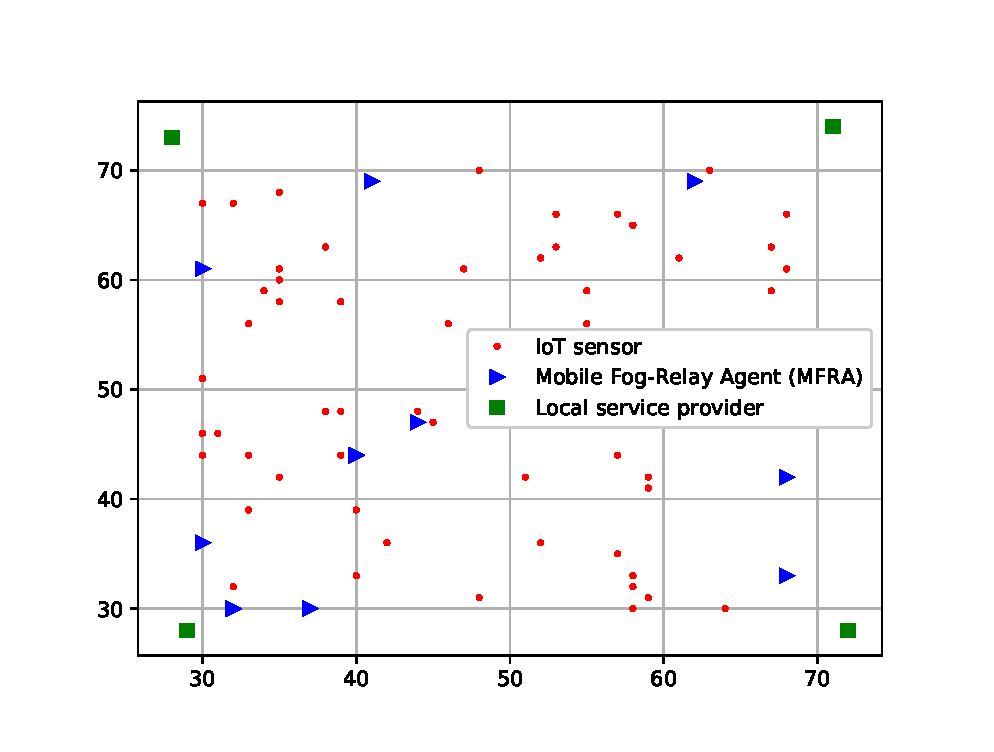
\includegraphics[width=3.6in]{random_deploy.eps}
 %where an .eps filename suffix will be assumed under latex,
% and a .pdf suffix will be assumed for pdflatex; or what has been declared
% via \DeclareGraphicsExtensions.
\caption{Simulation instance using 60 IoT sensors, 10 MFRAs, and 4 local service providers.}
\label{random_deploy}
\end{figure}

\begin{figure}[!t]
\centering
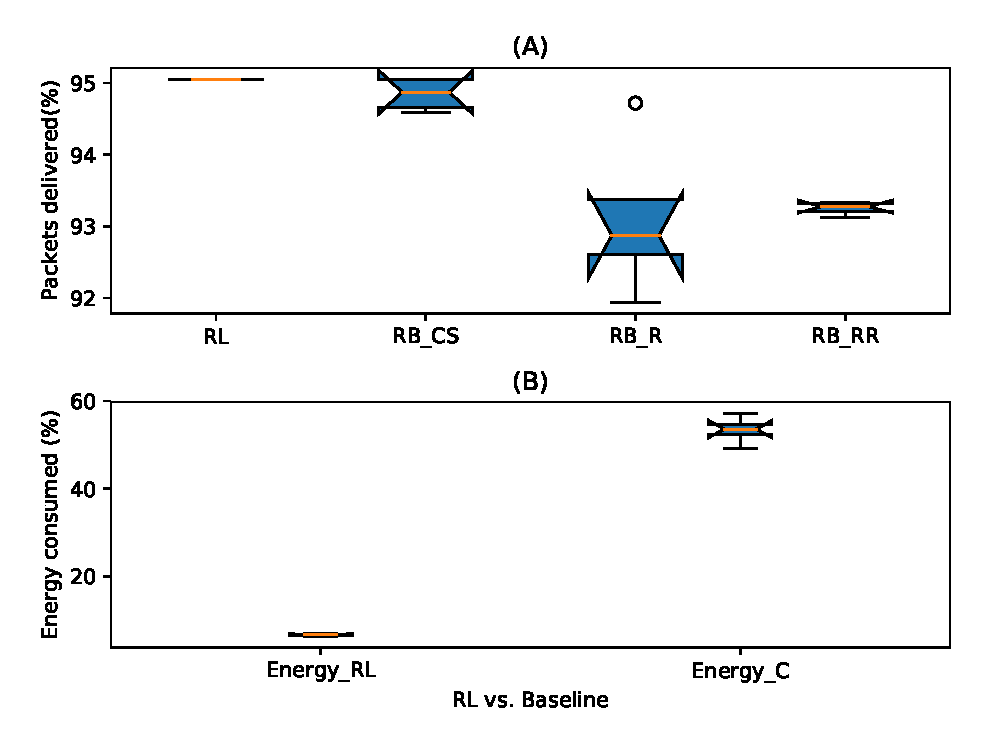
\includegraphics[width=3.6in]{2agentbaseline.eps}
 %where an .eps filename suffix will be assumed under latex,
% and a .pdf suffix will be assumed for pdflatex; or what has been declared
% via \DeclareGraphicsExtensions.
\caption{Comparison of RL with baselines over 50 runs in a 2 agents environment (a) Percentage of packets successfully transmitted by the active fog relay agents,  (b) Percentage of energy consumed by the active fog relay agents.}
\label{2agent}
\end{figure}



\subsection{Energy utilization for 2 MFRAs}
Fig. \ref{2agent} (b) depicts the percentage of energy consumed by the active fog relay agents in the network. Our proposed approach out-performs the baseline by efficiently minimizing energy cost within the network. The RB-CS strategy was able to achieve a range between 7.5\% - 17.8\%, and a median of 11.2\%, performing better than the RB-R and RB-RR strategies, which achieved a range between 20.9\% - 38.6\% and 18.6\% - 44.6\%, and median of 28.9\% and 30.0\%, respectively. The proposed RL approach has the least variation with a median of about 2.3\%. This shows that the decentralized learning by agents within the system significantly improves its energy utilization. The agents can learn when not to be active in order to minimize energy cost. Overall, the performance of the proposed approach yields better results than the baseline.

\begin{figure}[!t]
\centering
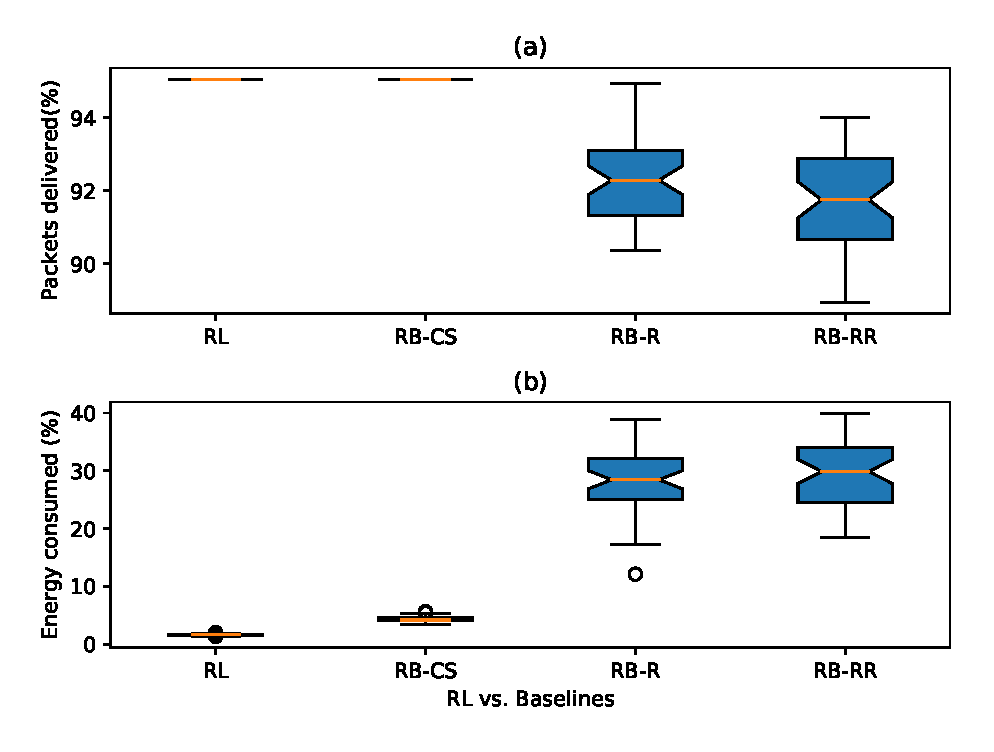
\includegraphics[width=3.6in]{5agentbaseline.eps}
 %where an .eps filename suffix will be assumed under latex,
% and a .pdf suffix will be assumed for pdflatex; or what has been declared
% via \DeclareGraphicsExtensions.
\caption{Comparison of RL with baselines over 50 runs in a 5 agents environment (a) Percentage of packets successfully transmitted by the active fog relay agents,  (b) Percentage of energy consumed by the active fog relay agents.}
\label{5agent}
\end{figure}

\subsection{Communication performance for 5 MFRAs}
In Fig. \ref{5agent} (a), we show the percentage of packets successfully transmitted by the active fog relay agents when conveying messages from IoT sensors to a remote destination. We observe that both our RL approach and RB-CS successfully transmitted about 95\% packets. The improved performance of RB-CS strategy may be due to the increase in redundant relays within the network. However, both the RB-R and RB-RR strategies perform poorly with the percentage of successfully transmitted packets ranging between 90.4\% - 94.8\% and 89.0\% - 94.0\%, and median of 92.3\% and 91.8\%, respectively. Furthermore, we observe higher variability in the RB-R and RB-RR strategies, as compared to the RL approach and the RB-CS strategy.

\subsection{Energy utilization for 5 MFRAs}
Fig. \ref{5agent} (b) shows the percentage of energy consumed by the active fog relay agents in a 5 MFRA-based IoT network. Our proposed approach out-performs the baseline by efficiently minimizing energy cost within the network. This is due to the fact that the agent learns to enter a passive mode and do nothing when there exist potential MFRA that can tranmit same message at a better QoS. However, the RB-CS strategy was able to achieve a good energy utilization with a median of 5.3\%, performing better than the RB-R and RB-RR strategies, ranging between 17.3\% - 39.0\% and 18.8\% - 40.4\%, and median of 28.9\% and 28.7\%, respectively. The proposed RL approach has the least variation with a median of about 1.7\%. This shows that the decentralized learning by 5 agents significantly improves its energy utilization. The agents can learn when not to be active in order to minimize energy cost. Overall, the performance of the proposed approach yields better results than the baseline.

\begin{figure}[!t]
\centering
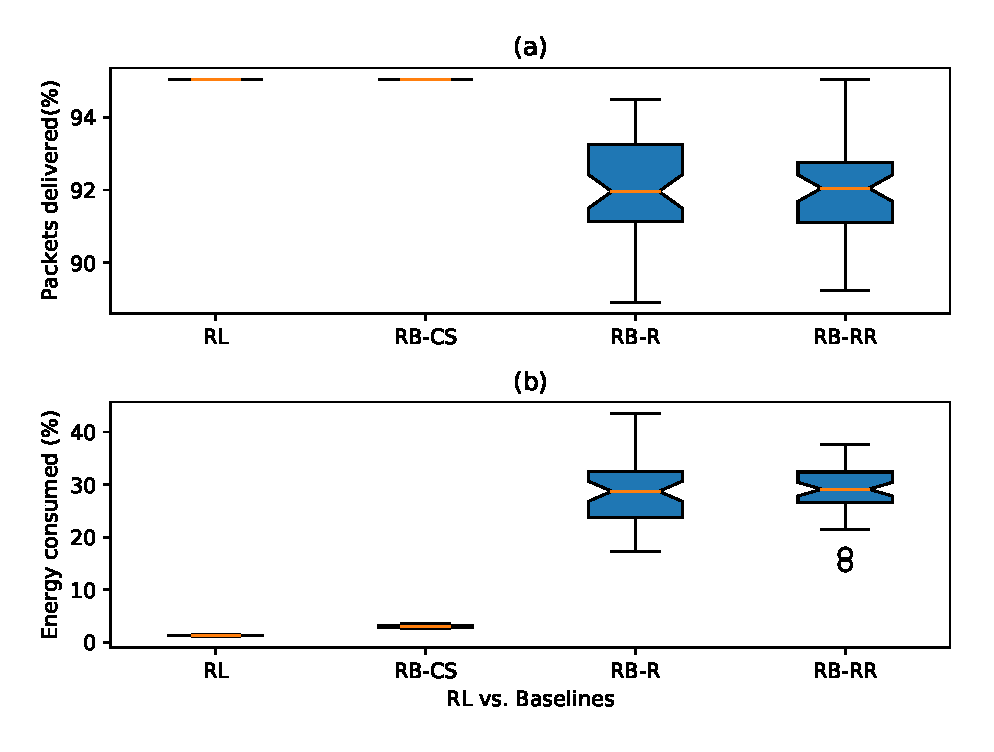
\includegraphics[width=3.6in]{10agentbaseline.eps}
 %where an .eps filename suffix will be assumed under latex,
% and a .pdf suffix will be assumed for pdflatex; or what has been declared
% via \DeclareGraphicsExtensions.
\caption{Comparison of RL with baselines over 50 runs in a 10 agents environment (a) Percentage of packets successfully transmitted by the active fog relay agents,  (b) Percentage of energy consumed by the active fog relay agents.}
\label{10agent}
\end{figure}

\subsection{Communication performance for 10 MFRAs}
In Fig. \ref{10agent} (a), we show the percentage of packets successfully transmitted by the active fog relay agents when conveying messages from IoT sensors to a remote destination. We observe that both our RL approach and RB-CS successfully transmitted about 95\% packets. The improved performance of RB-CS strategy may be due to the increase in redundant relays within the network as in the 10 MFRA network. However, both the RB-R and RB-RR strategies perform poorly with the percentage of successfully transmitted packets ranging between 89.9\% - 94.5\% and 89.2\% - 95\%, and median of 91.9\% and 92.1\%, respectively. Furthermore, we observe higher variability in the RB-R and RB-RR strategies, as compared to the RL approach and the RB-CS strategy, which converged.

\subsection{Energy utilization for 10 MFRAs}
Fig. \ref{10agent} (b) shows the percentage of energy consumed by the active fog relay agents in a 10 MFRA-based IoT network. Our proposed approach out-performs the baseline by efficiently minimizing energy cost within the network. This is due to the fact that the agent learns to enter a passive mode and do nothing when there exist potential MFRA that can tranmit same message at a better QoS. However, the RB-CS strategy was able to achieve a good energy utilization with a median of 3.5\%, performing better than the RB-R and RB-RR strategies, ranging between 17.2\% - 43.7\% and 21.5\% - 38.0\%, and median of 28.9\% and 29.2\%, respectively. The proposed RL approach has the least variation with a median of about 1.5\%. This shows that the decentralized learning by 10 agents significantly improves its energy utilization. The agents can learn when not to be active in order to minimize energy cost. Overall, the performance of the proposed approach yields better results than the baseline.



\section{Conclusion and Future works}
In this paper, we apply a decentralized q-learning algorithm on a multi-agent fog-based IoT system where multiple MFRAs compete to relay information in a highly dynamic environment, where long source to destination distances and obstacles considerably contribute to communication outages within the network. Furthermore, in an attempt to improve the communication performance, the MFRAs change positions which increases energy cost. As such, we carry out a comparative study and perform 50 experiments which show that our RL-based approach outperforms the three baselines (both in QoS and energy utilization) with lesser variations. Moreover, there was significant improvement in communication performance and energy utilizations as more MFRAs were deployed, which can be justified by addition of redundant agents to improve overall QoS. Intuitively, for the other approaches to match the performance of our proposed approach, more MFRAs must be deployed in the network. Overall, the performance of the proposed approach yields
better results than the baselines. Our future work will take into consideration fairness and latency within the fog-based IoT system. 




\ifCLASSOPTIONcaptionsoff
  \newpage
\fi

%\newpage

% trigger a \newpage just before the given reference
% number - used to balance the columns on the last page
% adjust value as needed - may need to be readjusted if
% the document is modified later
%\IEEEtriggeratref{8}
% The "triggered" command can be changed if desired:
%\IEEEtriggercmd{\enlargethispage{-5in}}

% references section

% can use a bibliography generated by BibTeX as a .bbl file
% BibTeX documentation can be easily obtained at:
% http://mirror.ctan.org/biblio/bibtex/contrib/doc/
% The IEEEtran BibTeX style support page is at:
% http://www.michaelshell.org/tex/ieeetran/bibtex/
%\bibliographystyle{IEEEtran}
% argument is your BibTeX string definitions and bibliography database(s)
%\bibliography{IEEEabrv,../bib/paper}
%
% <OR> manually copy in the resultant .bbl file
% set second argument of \begin to the number of references
% (used to reserve space for the reference number labels box)
\begin{thebibliography}{1}
\bibitem{Omoniwa2018}
B. Omoniwa, R. Hussain, M. A. Javed, S. H. Bouk and S. A. Malik, "Fog/Edge Computing-based IoT (FECIoT): Architecture, Applications, and Research Issues," in IEEE Internet of Things Journal.

\bibitem{BenMimoune2017}
A. BenMimoune and M. Kadoch, "Relay Technology for 5G Networks and IoT Applications," Internet of Things: Novel Advances and Envisioned Applications, vol. 25, pp. 3-26, April 2017.

\bibitem{Chiangh2016}
M. Chiang and T. Zhang, ``Fog and IoT: An Overview of Research Opportuinities,'' IEEE Internet of Things, vol. 3, no. 6, pp. 854-864, Dec.
2016.

\bibitem{OmoniwaRelay2018}
B. Omoniwa et al., "An Optimal Relay Scheme for Outage Minimization in Fog-based Internet-of-Things (IoT) Networks," in IEEE Internet of Things Journal.

\bibitem{Simiscuka2018}
A. A. Simiscuka and G. Muntean, "A Relay and Mobility Scheme for QoS Improvement in IoT Communications," 2018 IEEE International Conference on Communications Workshops (ICC Workshops), Kansas City, MO, 2018, pp. 1-6.

\bibitem{Alsharoa2018}
A. Alsharoa, X. Zhang, D. Qiao and A. Kamal, "An Energy-Efficient Relaying Scheme for Internet of Things Communications," 2018 IEEE International Conference on Communications (ICC), Kansas City, MO, 2018, pp. 1-6.

\bibitem{Manzoor2018}
A. Manzoor, P. Porambage, M. Liyanage, M. Ylianttila and A. Gurtov, "DEMO: Mobile Relay Architecture for Low-Power IoT Devices," 2018 IEEE 19th International Symposium on "A World of Wireless, Mobile and Multimedia Networks" (WoWMoM), Chania, 2018, pp. 14-16.

\bibitem{Lv2018}
T. Lv, Z. Lin, P. Huang and J. Zeng, "Optimization of the Energy-Efficient Relay-Based Massive IoT Network," in IEEE Internet of Things Journal, vol. 5, no. 4, pp. 3043-3058, Aug. 2018.

\bibitem{Kawabata2017}
H. Kawabata, K. Ishibashi, S. Vuppala and G. T. F. de Abreu, "Robust Relay Selection for Large-Scale Energy-Harvesting IoT Networks," in IEEE Internet of Things Journal, vol. 4, no. 2, pp. 384-392, April 2017.

\bibitem{Behdad2018}
Z. Behdad, M. Mahdavi and N. Razmi, "A New Relay Policy in RF Energy Harvesting for IoT Networks—A Cooperative Network Approach," in IEEE Internet of Things Journal, vol. 5, no. 4, pp. 2715-2728, Aug. 2018.

\bibitem{Gueriau2018}
M. Gueriau and I. Dusparic, "SAMoD: Shared Autonomous Mobility-on-Demand using Decentralized Reinforcement Learning,"  1558-1563. 10.1109/ITSC.2018.8569608.

\bibitem{Wilhelmi2017}
F. Wilhelmi, B. Bellalta, C. Cano and A. Jonsson, "Implications of decentralized Q-learning resource allocation in wireless networks," 2017 IEEE 28th Annual International Symposium on Personal, Indoor, and Mobile Radio Communications (PIMRC), Montreal, QC, 2017, pp. 1-5.

\bibitem{Azari2018}
A. Azari and C. Cavdar, "Self-organized low-power IoT networks: A distributed learning approach," arxiv


\end{thebibliography}


% that's all folks
\end{document}


